 \mysection{The Forgotten}{arcana-forgotten}

\flavor{
  Four Gods wait on the windowsill \\
  Where once eight Gods did war and will, \\
  And if the gods themselves may die, \\
  What does that say for you and I? \Tilde On the Rainslick Precipice of Darkness
}


Three aspects allow you to control the Forgotten:  \mybold{Remembrance}, \mybold{Sovereignty}, and \mybold{Potential}:

\mybullet{
    \item  Remembrance allows you to recall the name of one of the Abandoned, and call them forth from the abyss to do your bidding.
    \item  Sovereignty dictates how many times you can summon one of the Obliterated before you have to rest.  It also governs how many Abandoned you can have summoned at any given time.
    \item  Potential is the power of the Forgotten (Abandoned and Obliterated) under your control
}

The Forgotten will obey you and only you (though some Demons or Abandoned may try to twist your words or intent), but if you are Knocked Out, catch the Vapors, or are otherwise incapacitated, effects may vary (Arbiter's choice) ...

The Forgotten do not speak Acheron - knowledge of their "native" language (Archaic, Seraphic, or Fiendish) is necessary to command them.  You may not summon a creature whose language you cannot speak.  

\cbreak

\mysubsection{The Obliterated}{forgotten-obliterated}

You can summon one of the Obliterated to spy, fight, or distract on your behalf.  You can do this a number of times equal to your Sovereignty before you must rest.  The type of Obliterated you can summon depends on which Anamnesis you know (Beasts, Elements, or Damned).  The Obliterated use your Awareness \UD to Fight and Guard; if they are reduced to 0 Health, or if your Awareness is exhausted, they immediately adjourn. The Obliterated appear as spectral and indeterminate forms; they appears to always be shifting in appearance, and exude a ghostly and ethereal mist or smoke (they clearly do \mybold{not} look normal!)



  \begin{center}
  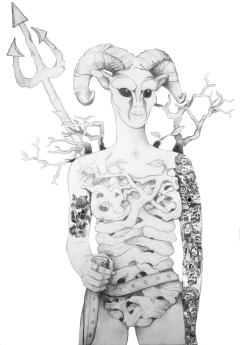
\includegraphics[scale=.5]{Spriggan}
  \end{center}


\myhighlight{Anamnesis of the Beasts}{forgotten-anamnesis-beasts}

Choosing this Virtue allows you to summon a phantom animal to assist you.  The beast will remain under your control for as long as you maintain Concentration, or until Days have elapsed.  This beast can be a mundane sort, or it can be a Zoological Monster (see below).  Beasts only understand \mybold{Archaic}.

\myital{Mundane Beasts:}  The creature will respond to your mental commands, provided they are Close or Nearby to you.  They can follow simple instructions ("get the key on the desk", "chew through these ropes", "spy on that man") but not more complex ones ("pick the lock").  The beast cannot speak. It can be sent on missions a number of kilometers away equal to your Potential. You can see what they see and hear what they hear for as long as you Concentrate. If they take any damage, or if you stop concentrating, they will immediately Adjourn (disappear).

\myital{Monstrous Beasts:}  In addition to animals of a mundane sort, you can also summon a Zoological creature(s) whose combined \HD do not exceed your Potential (if your Potential were 3, for example, you could summon 3 1 \HD beasts, or 1 3 \HD beast, etc).  These creatures will fight on your behalf for as long as you maintain Concentration.  The beasts use your Awareness \UD to Fight and Guard; if they are reduced to 0 Health, or if your Awareness is exhausted, they immediately Adjourn.


\mytable{X c}{
\thead{Beast} & \thead{Potential} \\
}{
    Swarm & * (varies) \\
    Giant Toad & 1 \\
    Troglodyte & 1 \\
    Giant Spider & 2 \\
    Lizard Man & 2 \\
    Giant Lizard & 3 \\
    Dire Wolf & 3 \\
    Giant Ant & 3 \\
    Toad Man & 3 \\
    Giant Centipede & 4 \\
    White Ape & 4 \\
    Giant Snake & 4 \\
    Giant Beetle & 5 \\
    Pteranodon & 5 \\
    Cave Bear & 5 \\
    Salamander & 5 \\
    Triceratops & 6 \\
    Sabertooth Tiger & 6 \\
    Allosaurus & 6 \\
    Plesiosaurus & 7 \\
    Tyrannosaurus Rex & 8 \\
}

\cbreak

\myhighlight{Anamnesis of the Elements}{forgotten-anamnesis-elements}

Choosing this Virtue allows you to parlay with an elemental creature to assist you.  The elemental will remain under your control for as long as you maintain Concentration, or until Hours have elapsed.  This elemental can be a "mundane" sort (an Imp), or it can be a Lesser or Greater Elemental (see below).  Elementals only understand \mybold{Seraphic}.

\myital{Imps:}  The Imp will respond to your mental commands, provided they are Close or Nearby to you.  The Imp is an elemental of a single type (fire, water, smoke, etc) and can take any form you wish, but it can't have a total size in meters greater than your Potential (for instance, if your Potential were 2, it could not be more than 2 meters tall or 2 meters wide). Imps can't cause any damage directly, though they can affect the environment appropriate to its type.  For instance, you could summon a Fire Imp to run into a room to set something alight, or summon a Smoke Imp to stand in a doorway and hide something.   It can follow simple instructions ("jump into the hay (Fire)", "douse the fire (Water)", "blow out the torches (Air)") but not more complex ones ("burn the book the lich is carrying").  The Imp cannot speak. The Imp can't move further than Far Away from you.  Unlike Beasts, you cannot see what they see or hear what they hear (they make terrible spies). If they take any damage, or if you stop concentrating, they will immediately Adjourn (disappear).

\myital{Elementals}:  In addition to Imps, you can also summon Lesser or Greater elementals whose combined \HD do not exceed your Potential.  The elemental will fight on your behalf for as long as you maintain Concentration.  The elementals use your Awareness \UD to Fight and Guard; if they are reduced to 0 Health, or if your Awareness is exhausted, they immediately Adjourn.


\mytable{X c}{
\thead{Elemental} & \thead{Potential} \\
}{
    Lesser & 5 \\
    Greater & 7 \\
}

\newpage

\myhighlight{Anamnesis of the Damned}{forgotten-anamnesis-damned}

Choosing this Virtue allows you to wrest a Demon from the depths of Hell to obey you.  The Demon will remain under your control for as long as you maintain Concentration, or until Minutes have elapsed.  This Demon can be a "mundane" sort (a Gremlin), or it can be a Demonic monster (see below).  Demons only understand \mybold{Fiendish}.
All Demons are Unhallowed. 


\myital{Gremlins:}  Gremlins can be summoned somewhere Close or Nearby to  you.  Gremlins can only cause havoc and chaos; you can partially guide them, but generally they are under the control of the Arbiter.  When they are summoned they immediately run in different directions (but won't move further than Far-Away from you) and cause as many problems as they possibly can - unbuckle belts, set things on fire, cut ropes, smash pottery, scream and kick in the middle of the floor, etc.  They may or may not follow instructions (Arbiter's discretion.  If you're stuck, roll a die and have them react randomly).  You can see what they see and hear what they hear, but it's generally unpleasant to do so.  You summon a number of Gremlins equal to your Potential.  If they take any damage, or if you stop concentrating, they will immediately Adjourn (disappear).

\myital{Devils:}  In addition to Gremlins, you can summon various types of Devils whose combined \HD do not exceed your Potential (if your Potential were 3, for example, you could summon 3 1 \HD Dretch, or 1 3 \HD Vrock, etc).  These Devils take no damage from iron weapons or from spells \mybold{not}  of the Entropy paradigm. Seeing a Devil prompts a Sanity check (including for Allies!).  See the Bestiary for further information on Demons.

\mytable{X c}{
\thead{Demon} & \thead{Potential} \\
}{
    Dretch & 1 \\
    Vrock & 3 \\
    Slaad & 5 \\
    Naga & 7 \\
    Balor & 9 \\
}

\cbreak

\mysubsection{The Abandoned}{forgotten-abandoned}

In order to summon the Abandoned, you call them forth using their True Name - represented by your Remembrance.  Remembrance is either bound or unbound.  You can use an unbound Remembrance to recall the name of \myital{any} Abandoned (essentially, tell the Arbiter the name of the Abandoned you wish to call forth when you're ready to summon them).  From then on, that point of Remembrance is now bound to that Abandoned, and you can only use it to summon that specific Abandoned. You can add additional unbound Remembrance points when you gain levels; alternately, the Arbiter may place the True Names of various Abandoned as treasure in the game.  Learning the True Name of one of the Abandoned from treasure in this way counts as a "bound" Remembrance.

Any attacks against the Abandoned automatically succeed.  They can take up to your Potential x 5 points of damage before they Adjourn (so if you had 3 Potential, they would be able to take 15 points of damage).  If an Abandoned adjourns for any reason during a Session, it will not return until the next Session. You can have a number of Abandoned summoned equal to your Sovereignty at any time, but be warned - Abandoned are fickle and proud spirits, and may not cooperate with other Abandoned.

Unless otherwise noted, Abandoned will not Adjourn until the end of the Session unless they can be somehow convinced to do so (or if they take enough damage to force them to Adjourn).  The Abandoned have memory and personalities, and won't take kindly to being forced to Adjourn by "killing" them!

Below are the 12 Archons, Seraphs, and Fiends who can be summoned via their true name.  This is by no means a complete list - feel free to work with an Arbiter to create different Abandoned.  Archons speak Archaic; Seraphs speak Seraphic; and Fiends speak Fiendish.


\newpage

\ed{Lots of influence from Skerple's mind-blowing \href{https://coinsandscrolls.blogspot.com/2019/10/osr-glog-based-homebrew-v2-many-rats-on.html}{GLOG Homebrew v.2}}



\mysubsection{The Archons}{forgotten-archons}


\myhighlight{Big Mac, "Good Time Guy"}{abandoned-big-mac-good-time-guy}

Big Mac crashes through a window or door and drunkenly hugs the first person he sees. He appears as a portly robed monk with a tankard of beer and a rosy complexion.  He is totally smashed and very happy.  

Unless Big Mac is at a party (at minimum, drinks and 2 happy people) he will leave the way he came in with an "Irish goodbye" (adjourning).  If there's a party, he will continue to drink from his tankard (which never gets empty), tell tall tales, reminisce, propose mad schemes, sing songs in all languages, provide terrible advice, and sometimes throw up.  He cheers up any low-class social event and scandalizes anyone tasteful. Big Mac can find a number of items equal to your Potential for you, provided they are party related.  Examples:  more beer, a safe place to crash, a person of negotiable virtue, Pooka, narcotics, musicians.  He can remove Toxins or Drunkenness from a number of people equal to your Potential.

\myhighlight{Bon Chapeau, Hat of Marvels}{abandoned-bon-chapeau-hat-of-marvels}

Bon Chapeau enters with a burst of light on a target's head up to a distance of Far Away.  It appears a magnificent hat, crown, turban, etc. depending on how Bon Chapeau is feeling that day (but it will always match the wearer's garments).  

If the wearer is under the effect of a Mind spell when the hat appears on their head, the spell is immediately broken.  If someone attempts to cast a Mind spell against the wearer, the spell rebounds on the caster. 

The hat can hear the wearer's thoughts, and will tell them to you if asked.  It can also judge fashion shows and tell you if an article of clothing is a knock off or not.

\myhighlight{Bufo, the Lickable Toad}{abandoned-bufo-the-lickable-toad}

A fat green toad the size of a housecat hops in.  He has yellow eyes and many warts, and speaks in a booming croak. 

Anyone who licks Bufo must make a Sanity check; if they succeed, they can invoke one of the following effects:
\mylist {
\item they can restore all Intangible Stats to their \MAX
\item they can heal their Flesh fully, or
\item they can heal their Grit fully
}

Bufo doesn't like being licked.  There is a cumulative 1 in 6 chance that anyone who that licks him will gain no positive effect (i.,e.  on the second lick, there is a 2-in-6 chance it will have no positive effect, a 3rd 3-in-6, etc).  Once this number hits 6-in-6, no further beneficial effects can occur for the remainder of the Session.

Objects swallowed by Bufo enter Hammerspace until he adjourns, when he will spit them back out.  He'll only swallow things that look delicious (but he's easily tricked).  The object swallowed can't be bigger than he is.



\myhighlight{Gemma, Translator of Mysteries}{abandoned-gemma-translator-of-mysteries}

A thin, tired woman with wiry hair appears wherever you're not looking.  Gemma can speak and translate any language (living or dead), and will translate for you in real time.  Gemma won't speak or translate blasphemies (which are basically things written in Fiendish or Seraph).  If Gemma is reading by the light of the sun, she'll prepare a full allegorical and contextual translation.  She can't (or refuses to) write.  While Gemma is Close to you, you can't be Befuddled (and ends any Befuddled effect on you if applicable).

\myhighlight{István, the Lost}{abandoned-istván-the-lost}

A tired, middle-aged man with blue eyes shuffles in politely.  Anyone who talks to István will give him directions to any place you name.  Directions given will be to the best of the person's knowledge, and can include the location of treasure, traps, hazards, patrols, etc. etc.  Ask a peasant how to get to the moon and he'll shrug and suggest a mountain; ask the Grand Archmage of the Isle of Carcosa and you might get a very different answer.  


\myhighlight{Judyth, the Tiebreaker}{abandoned-judyth-the-tiebreaker}

Judyth is a floating stone sphere about bowling ball sized, carved in the shape of a human head.  She floats down from the ceiling and speaks with a decisive, stern voice.  If two objects, items, ideas, or issues are presented to Judyth (along with some criteria for judging) she will judge their merits. For example, you could ask "Which of these gems is most valuable?", "Which of my friends loves me most?" or "Which of these two mushrooms is tastes better?" Judyth can't answer questions that aren't local and immediate:  "Which country will win the war?" or "Which hallway did the thief run down?" aren't allowed, for example.  If Judyth is presented with a paradox, she will immediately adjourn in a logic bomb that deals your Potential x 3 damage to everyone Close (Save for half).

\myhighlight{Mikhael, the Justifier}{abandoned-mikhael-the-justifier}

A middle-aged, completely bland man enters with a shuffle.  You can't really describe him further than that; his appearance seems to be easily forgotten.  In a low and soothing voice. Mikhael will assist anyone in justifying any plan (or crime).  People who talk to Mikhael are freed of any guilt or doubt.  Mikhael has no secret knowledge, but hints vaguely at schemes by people in power (kings, religious leaders, etc).  

Any arrows or projectiles aimed at Mikhael or anyone Close to him automatically miss (whether they are Allies or Monsters)


\myhighlight{Mon Signor, the Deliverer}{abandoned-mon-signor-the-deliverer}

A bellboy comes running in with a patter of feet.  He hands you a package that contains d6 \UD of Provisions, waits for a tip (doesn't always get one), and then runs off - immediately adjourning.  The Provisions are always weird - a little too warm, a little too salty, a little too spicy, etc.  You can hand Mon Signor any item and it will be returned to you the next time he is summoned as if no time has passed (this item exists outside of Hammerspace, and can be the size of a human body)

\myhighlight{Randy.  Just Randy}{abandoned-randy-just-randy}

A pop, a short scream, and Randy falls down from the ceiling.  He is an acned teenage human with brown hair and a torn blue robe.  Randy was once a wizard's apprentice; a botched spell trapped him in a pocket dimension where he lives on, immortal and extremely confused. He is perpetually being dragged into combat, danger, dismemberment, and extremely awkward situations. 

Randy will sort-of obey you for the Session, but he is only an immortal teenager. He's awful at everything. If you want, you can direct any physical attack against you to Randy instead.  If you have more than 3 Potential, Randy's efforts are accompanied by appropriately dismal music.  Randy insists on an honorific i.e. "Randy the Magnificent", "Randy the Stupendous", etc. but no one ever calls him that.

\myhighlight{Smök, the Grey Messenger}{abandoned-smök-the-grey-messenger}

Smök seeps in through cracks in the floor and ceiling, appearing as a grey flag flapping in the wind.  You can give Smök a message containing a number of words up to your Potential or an object smaller than an apple - the apple or message will vanish, and Smök will move as quickly as an arrow (325km/h), to bring the item to location or person you designate.  If Smök can't reach the target by the end of the Session, it will drop the item somewhere along the quickest path.


\myhighlight{VVulf, Trapfinder}{abandoned-vvulf-trapfinder}

The sound of a trap springing shut echoes through the room, and a starving 3-legged wolf appears before you, fur matted with blood.  VVulf can detect any traps Nearby until he adjourns.  Zoological animals feel affinity with VVulf - provided combat has not been initiated, the Monster will not attack if they fail a Morale check.  VVulf is able to talk to mundane animals and ask simple questions (and receive basic answers).  VVulf immediately adjourns if anyone Nearby exhibits cruelty towards an animal.

\myhighlight{Weeble, the Wobbling Stone}{abandoned-weeble-the-wobbling-stone}

A stone egg of a rotund, happy man with a cheerful grin appears in your hand.Anyone holding Weeble cannot be knocked Prone or Stunned.  If you would fall into a pit or off a cliff, Weeble wobbles you back to safety at the last possible moment - but Weeble can't help you if the bridge collapses or your boat explodes or what-have-you.  If you had Weeble to any liquid (soup, wine, etc) it will neutralize any Toxins inside.



\mysubsection{The Fiends}{forgotten-fiends}


\myhighlight{Al Ana, the Slaughtercaller}{abandoned-al-ana-the-slaughtercaller}

A red stone carved with a snarling tiger biting its own tail appears with a sizzle in your hand.  All weapon damage dealt within a Close or Nearby radius of Al Ana is doubled (from Allies and Monsters).  If you throw Al Ana using your \DEX, it will deal your Potential in damage (i.e. if your Potential is 4, it will deal 4 damage on a successful hit) and return to your hand at the bottom of the Moment.  Al Ana growls before ambushes, making you immune to Surprise.

\myhighlight{Ben Sidhe, Singer of Death}{abandoned-ben-sidhe-singer-of-death}

A spectral woman with long, streaming hair boils up from the floor in a white mist.  She wears a grey cloak over a green dress, and her eyes are red from weeping.  She immediately begins wailing.  All creatures Nearby (except you) take your Potential in damage.  The damage increases by +1 and repeats at the top of each Moment after the first until a Save vs. Doom is made.  Ben Sidhe cannot be silenced and will not stop weeping until she adjourns.  She will always remain Close to you.

\myhighlight{Diviseré, the Universal Chisel}{abandoned-diviseré-the-universal-chisel}

A simple iron chisel with a wooden handle appears in your hand.  Diviseré can separate any two layers.  You could separate skin from muscle, gold foil from wood, rust from iron, or the bark from a tree. You can't separate things that are not fused, so Diviseré couldn't chisel the armor off a warrior or the nose off a statue (at least, not any more than a normal chisel could). Diviseré can separate things joined by Brahe's Efficacious Sealant.  Diviseré can't speak


  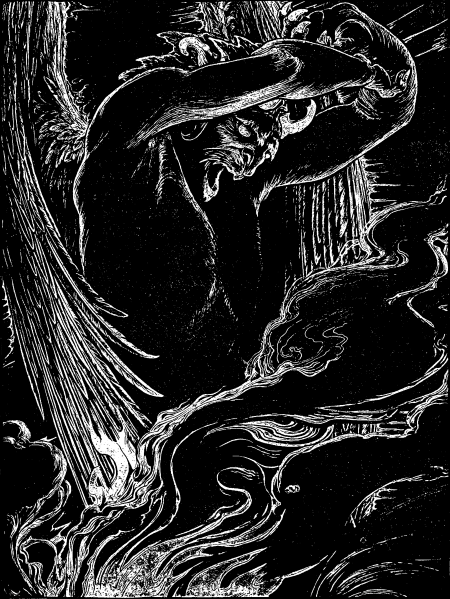
\includegraphics[scale=.45]{Demon}

\myhighlight{Doppel, the Mirror}{abandoned-doppel-the-mirror}

An identical duplicate (save for some subtle detail, like a different eye color) of you steps from your shadow.  Doppel will act as directed by you, including very complex tasks (though Doppel can't improvise).  Doppel can't deal damage or cast spells, but can invoke minor Illusions to make it appear that it can.  Doppel is unable to speak.

\myhighlight{Gitgud, the Taunter}{abandoned-gitgud-the-taunter}

A skinny monkey in torn robes appears with a low whistle.  Gitgud has a toothy, sneering grin and tiny red eyes.  Gitgud will taunt any target you tell it to with capers, jeers, wails, and jokes.  He is really distracting and annoying.  The target must Save vs Doom or immediately attack Gitgud, who will run away to taunt from a safe distance.  He can climb and perform simple tasks with a monkey's patience and skill.

\myhighlight{Grendel, the Helping Hand}{abandoned-grendel-the-helping-hand}

A blue-green arm and hand drops from the sky with a wet thud.  The arm can be stuck to flesh and acts as an extra limb.  On a willing target, Grendel grants an additional Unarmed attack each Moment that deals your Potential in damage (\MAX 6).  Use the target's \FOC instead of \VIG or \DEX when they make their Fight roll.  It can carry a shield or a lantern, or assist with climbing or swimming (+2 to the roll), but cannot wield a weapon.  If attached to an unwilling creature, Grendel will punch them in the nearest vulnerable spot, deals your Potential in damage (\MAX 6).  The arm detaches with a pop;  it can be stuck to a number of creatures equal to your Potential every Session.

\myhighlight{Grimalkin, Ruler of the Weak}{abandoned-grimalkin-ruler-of-the-weak}

A purring grey cat with yellow eyes comes curling out from the shadows between your legs.  Grimalkin is an asshole; she'll ignore what your asking her, get into trouble, and generally be a nuisance.  However, she can also do the following:

\mylist {
    \item Eat a Curse (see \mylink{Hekaphage}{occultism-hekaphage});
    \item Turn any die roll that hits the table into a natural 1;
    \item Knock a single die off the (real world) table. The roller gets a re-roll.
}

She can perform any of those abilities a number of times equal to your Potential, at which point she adjourns.

\myhighlight{Lucertola, the Taster}{abandoned-lucertola-the-taster}

A sleek yellow lizard with a bright blue tongue appears around your neck.  Lucertola can taste the air and tell you about the source of odors, smoke, fog, etc.  If you give Lucertola a taste of food or drink, it can tell you whether or not its safe to eat or drink.  While you're wearing Lucertola you can breathe underwater, and you're immune to inhaled Toxins.

\myhighlight{Mirót, the Critic}{abandoned-mirót-the-critic}

A tinkling of glasses and a cleared throat herald a balding man in a tweed jacket, or woman of impeccable dress and haughty expression, who step out from a nearby doorway.  In either form, Mirót's eyes are milky white.  Mirót hates all works of art, and will move from room to room, destroying any artwork, carvings, decorations, or written works it can see (Grimoires and Fetishes not included).  This also includes objects that can create art - instruments, paints, paintbrushes, inks, and empty scrolls and papyri.  It won't ever attack a living creature, but can set things on fire with a touch.  Mirót is a blunt instrument - if prevented from entering a museum, for instance, it will burn the museum to the ground in order to destroy the art inside.  If an actual artist is present (musician, painter, sculptor, writer, scribe, etc) Mirót will hurl insults and epithet's at the artist in a non-ending stream of vitriol; all \RO and \RS attempts by the "victim" are at -4 as long as he or she is forced to endure the onslaught.  Mirót will adjourn if there is nothing around it to criticize, and nowhere else for it to go.


\myhighlight{Nyumbu, the Broken}{abandoned-nyumbu-the-broken}

A broken, skeletal mule with fire burning in its eye-sockets clatters in from behind you.  Nyumbu can carry up to 50 Significant Items for you and can travel over water and air as if it were solid ground.  It can only walk in a straight line and can't jump - you could lead Nyumbu up to a cliff face and over a chasm, but unless there were a cliff of equal height on the other side, it will remain hovering in air.  As long as your hand is on Nyumbu's bridle, it conveys the ability to walk on water and air to you as well.  When Nyumbu adjourns, everything it was carrying falls on the ground.  If Nyumbu is ever struck for damage by someone Close, it will immediately kick at the attacker and automatically deal damage equal to your Potential; regardless of the range of the striker, Nyumbu will immediately adjourn if struck, dropping what it was carrying (and potentially yourself) onto the ground.

\myhighlight{Orobas, the Moneychanger}{abandoned-orobas-the-moneychanger}

A squashed and twisted homonculous with a huge gut and tiny limbs appears in a puff of cigar smoke.  Orobas sports a top hat, monocle, and cigar but has not neck or eyes to speak of.  Orobas will eat any coins you give to it, and spit them back up at your request at any point (even if summoned years later).  These coins exist outside of Hammerspace.  Orobas will only eat Iron, Silver, or Gold coins - not jewelry, gems, or anything else.  Orobas can accurately state the amount of money a person is carrying at any given time, or the number of coins (and types) in a pile.  He can give you "business advice", but it almost always involves killing someone.


\myhighlight{Pocong, the Piper}{abandoned-pocong-the-piper}

A tiny grey cloth effigy of you with strange, wet-looking eyes appears in a glimmer of light.  As long as Pocong is Close to you, you automatically pass any Saves vs Doom.  Pocong can't move on its own.  If the effigy is moved away from you to somewhere Nearby, or adjourns by taking damage, you must Save vs. Doom (not automatic!) or immediately be brought to 0 Flesh, prompting a \DEATH roll.



\mysubsection{The Seraphim}{forgotten-seraphim}


\myhighlight{Ada, the Calculator}{abandoned-ada-the-calculator}

A young woman with black hair and expensive Victorian garb appears from somewhere behind you.  Ada can measure the exact distance between two points (provided one of them is within sight) and immediately know the direction of true north no matter where she is.  She can rapidly calculate any number of items provided they are separated from one another (she couldn't count the number of coins in a pile, for instance, unless that pile was separated into individual coins).  As long as Ada remains Close to you, you automatically succeed on all Skill:Math checks.



\myhighlight{Beatrix, the Story Teller}{abandoned-beatrix-the-story-teller}

A very old woman in clean Victorian clothes enters with a polite knock and a quiet shuffle.  She carries an empty scabbard and a book tucked into an apron pocket.  If a fight breaks out with Beatrix present, she summons a rocking chair, pulls out the book, sits, and begins reading in a sweet and mesmerizing voice understood by all present.  Allies and Monsters alike must Save vs Doom at the top of each Moment or fall under the sway of Beatrix.  They will sheathe their weapons, sit at her feet, and listen to her story.

\myhighlight{Bíró, the Chronicler}{abandoned-bíró-the-chronicler}

A black quill of an unknown beast, half a meter in length, appears in your hand.  Bíró can't speak or see, but can hear excellently.  If you provide it ink (the blacker the better), Bíró will write the answers to any questions you ask as long as its heard the answer in the time since you summoned it.  It can transcribe conversations in perfect detail or tell you how many people entered a room, what they said, and when they left.

If anyone holds Bíró against your will, they must Save vs.  Doom or be reduced to 0 Health / Flesh.  If anyone holds Bíró with your permission, they must Save vs. Doom or become Charmed to you for Hours.  Either way,  Bíró adjourns if anyone other than you holds it.

\myhighlight{Crescendo, Choir of Heroes}{abandoned-crescendo-choir-of-heroes}

A quickly rotating cube appears above you, sending out rays of electric light with illumination as a torch, and begins chanting.  The chant fills the hearts of Allies with hope, courage, and the belief that if they can just see things through, everything will be OK.

Every Ally Close or Nearby to Crescendo is immune to Fear and anything that might cause despair (like the Wall of Gloom). If invoked during Combat,  Allied Hirelings all gain fanatic morale, and Allies regain your Potential in Grit at the top of each Moment (if they are at 0 Flesh, they still must roll their \DEATH however).  The Crescendo will adjourn at the end of your next Combat (or unless you tell them too).  

\myhighlight{Flux, the Hallowed Light}{abandoned-flux-the-hallowed-light}

A sphere of golden flame appears in a shimmer of light, shedding light as a torch.  Flux can flare and illuminate (briefly) an area from Close to Far-Away.  Sighted creatures in the area who aren't prepared must Save vs Doom or be Blinded for d4 Markovian.  The flare can even temporarily cancel magical darkness; it will re-emerge at 5m per Moment from its source.  Unhallowed won't approach Flux unless forced.

\myhighlight{Leroy, the Lucky Rose}{abandoned-leroy-the-lucky-rose}

A red rose with a silver stem appears in your hand.  Leroy inspires foolish confidence in anyone who wears him as a boutonnière.  The wearer will accept any risky but thrilling plan they are presented with. Provided the endeavor is risky enough (Arbiter's discretion), the wearer will receive +4 on all \RO or \RB attempts in pursuit of the plan.

\myhighlight{Pferdinana, the Sure Bet}{abandoned-pferdinana-the-sure-bet}

An ordinary-looking but tidily brushed grey mare appears with a clatter of hooves.  Pferdinana can speak to horses, but translates with snide remarks and uncomfortable, mocking laughter.  Pferdinana will permit you to ride her, but travels at a slow trot, sighing with boredom.  However, if she's asked to race another creature, she will win any race over any terrain, no matter how terrifying or improbable.  If your Potential is 5 or greater, Perfidnana will race inanimate objects, spells, the weather, etc.

\myhighlight{Sir Ector de Mares, First of the Snail Knights}{abandoned-sir-ector-de-mares-first-of-the-snail-knights}

A stooped man in a visored helmet, wearing antique armor, enters in through a door or window.  He creaks when he walks.  If called upon as a second in a duel, Sir Ector grants the following powers:

\mylist{
\item The duelist wins Init every Moment; 
\item The duelist cannot be disarmed; and 
\item The duelist gains +4 on all Fight and Guard rolls.
}

Sir Ector can tell true kings from false ones at a glance.


\myhighlight{Termagant, "My Old Lady"}{abandoned-termagant-my-old-lady}

When remembering Termagant, select a number of Hours from now when she should show up (immediately is fine).  At the designated time, a middle-aged woman of suitable race and appearance for the area enters screaming general accusations ("Coward!  Bastard!  Bitch!  etc.")  She grabs you and drags you away.  Termagant's appearance might be enough to convince guards or authority figures not to stop her, but if that fails she produces false documents, bribes, "proof", etc. - whatever it takes to get you out of the situation you're in short of violence.  She drags you out of sight and then promptly adjourns.  She'll only rescue you (not anyone else), and won't return for anything you left behind.  She can't heal you.  No barriers (magical or no) can hinder her, but she'll only take you to the next unlocked and unobserved area, then adjourn.

\myhighlight{Trismegistus, the Herald's Wand}{abandoned-trismegistus-the-heralds-wand}

Trismegistus appears in a stream of leaves and smoke as a shillelagh with a snake wrapped around it.  It will remove any a number of Diseases equal to your Potential.  Once it's reached its limit, it will hop along next to you and get into trouble.  Trismegistus can translate for any reptiles you might come across.

\myhighlight{Veritas, the Truth Teller}{abandoned-veritas-the-truth-teller}

An old man in fine robes or a beautiful young woman with no hair enters from somewhere behind you.  Veritas mutters like a madman, repeating meaningless phrases, snippets of conversation, and rocking back and forth.  As long as Veritas can see the tongue of a creature, it can tell if the creature is lying; if it detects a lie, it will lunge at them and remove their tongue.  The tongue stays in a pouch on its belt until it adjourns (at which point it returns to the tongueless victim with no ill effects).  Veritas can carry up to 25 Significant Items for you and will provide banal and useless advice if asked.


\myhighlight{Walden, the Quartermaster}{abandoned-walden-the-quartermaster}

A portly man with grey eyes and stained clothes enters from somewhere behind you.  You can ask Walden for up a number of items up to your Potential, and he will procure them for you.  The items must be mundane in nature and can't be specific:  "a pair of woolen trousers" or "a longsword" are OK, but "the cape of Felspex the Witch", "the magical blade of Aesop", or "a Grimoire containing the following spells" aren't possible.  If the item has a \UD attached (a quiver of arrows, for example) Walden will provide d4 \UD of the item (this means he can provide Heavy armor, but it only has d4 \UD, for instance).  If Walden adjourns, the items disappear.  Walden can identify who forged any weapon shown to him; when it was forged; and when the weapon was last used.






